\documentclass[11pt]{article}\usepackage[]{graphicx}\usepackage[]{color}
%% maxwidth is the original width if it is less than linewidth
%% otherwise use linewidth (to make sure the graphics do not exceed the margin)
\makeatletter
\def\maxwidth{ %
  \ifdim\Gin@nat@width>\linewidth
    \linewidth
  \else
    \Gin@nat@width
  \fi
}
\makeatother

\definecolor{fgcolor}{rgb}{0.345, 0.345, 0.345}
\newcommand{\hlnum}[1]{\textcolor[rgb]{0.686,0.059,0.569}{#1}}%
\newcommand{\hlstr}[1]{\textcolor[rgb]{0.192,0.494,0.8}{#1}}%
\newcommand{\hlcom}[1]{\textcolor[rgb]{0.678,0.584,0.686}{\textit{#1}}}%
\newcommand{\hlopt}[1]{\textcolor[rgb]{0,0,0}{#1}}%
\newcommand{\hlstd}[1]{\textcolor[rgb]{0.345,0.345,0.345}{#1}}%
\newcommand{\hlkwa}[1]{\textcolor[rgb]{0.161,0.373,0.58}{\textbf{#1}}}%
\newcommand{\hlkwb}[1]{\textcolor[rgb]{0.69,0.353,0.396}{#1}}%
\newcommand{\hlkwc}[1]{\textcolor[rgb]{0.333,0.667,0.333}{#1}}%
\newcommand{\hlkwd}[1]{\textcolor[rgb]{0.737,0.353,0.396}{\textbf{#1}}}%

\usepackage{framed}
\makeatletter
\newenvironment{kframe}{%
 \def\at@end@of@kframe{}%
 \ifinner\ifhmode%
  \def\at@end@of@kframe{\end{minipage}}%
  \begin{minipage}{\columnwidth}%
 \fi\fi%
 \def\FrameCommand##1{\hskip\@totalleftmargin \hskip-\fboxsep
 \colorbox{shadecolor}{##1}\hskip-\fboxsep
     % There is no \\@totalrightmargin, so:
     \hskip-\linewidth \hskip-\@totalleftmargin \hskip\columnwidth}%
 \MakeFramed {\advance\hsize-\width
   \@totalleftmargin\z@ \linewidth\hsize
   \@setminipage}}%
 {\par\unskip\endMakeFramed%
 \at@end@of@kframe}
\makeatother

\definecolor{shadecolor}{rgb}{.97, .97, .97}
\definecolor{messagecolor}{rgb}{0, 0, 0}
\definecolor{warningcolor}{rgb}{1, 0, 1}
\definecolor{errorcolor}{rgb}{1, 0, 0}
\newenvironment{knitrout}{}{} % an empty environment to be redefined in TeX

\usepackage{alltt}

\usepackage{amssymb}
\usepackage{amsmath}
\usepackage{bm}
\usepackage{graphicx}
\usepackage{hyperref}
\usepackage{url}
\usepackage{natbib}
\usepackage{epigraph}
\usepackage[utf8]{inputenc} % for UTF-8/single quotes from sQuote()

\usepackage{fancyvrb} % with VerbatimFootnotes, allow verb in footnotes
%\usepackage{listings}
\usepackage{array} % for ragged right table columns
% order of the next two matters
\usepackage[perpage,symbol]{footmisc}
\VerbatimFootnotes

\newcommand{\windows}{\textcircled{w}}
\newcommand{\code}[1]{{\tt #1}}
\newcommand{\flspecific}[1]{\emph{#1}}
%\bibliographystyle{ESA1009}

%\DeclareGraphicsExtensions{.jpg,.pdf,.mps,.png,.bmp}

% \setlength{\textwidth}{6.25in}
% \setlength{\textheight}{8.75in}
% \setlength{\evensidemargin}{0in}
% \setlength{\oddsidemargin}{0in}
% \setlength{\topmargin}{-.35in}
% \setlength{\parskip}{.1in}  
% \setlength{\parindent}{0.0in}  

% \numberwithin{equation}{chapter}
\pagestyle{headings}

\newcommand\R{{\sf R}}
\newcommand\Slang{{\sf S}}
\newcommand{\curRwver}{2013}

\newcommand{\curRver}{3.0.1}

\newcounter{exercise}
\numberwithin{exercise}{section}
\newcommand{\exnumber}{\addtocounter{exercise}{1} \theexercise \thinspace}

\newcommand{\prob}{\text{Prob}}


\sloppy
\title{Using \R\ to analyze continuous models (Lab 4)}
\date{\today}
\author{Steve Walker}}

%% TODO: hint about range change in log graph
%% mfcol(,)
%% ?
\IfFileExists{upquote.sty}{\usepackage{upquote}}{}
\begin{document}

\maketitle

\includegraphics[width=2.64cm,height=0.93cm]{../icons/cc-attrib-nc.png}

\begin{minipage}[b]{3in}
{\small Licensed under the Creative Commons 
  attribution-noncommercial license
(\url{http://creativecommons.org/licenses/by-nc/3.0/}).
Please share \& remix noncommercially,
mentioning its origin.}
\end{minipage}

Version: 2014-09-03 17:29:56
  
\addtocounter{section}{-1}

\section{Solving linear models}

We start simple, with the following bivariate linear model,
\begin{equation}
  \label{eq:2}
  \frac{d\bm x}{dt} = \bm A \bm x
\end{equation}
where the coefficient matrix, $\bm A$, is,
\begin{knitrout}
\definecolor{shadecolor}{rgb}{0.969, 0.969, 0.969}\color{fgcolor}\begin{kframe}
\begin{alltt}
\hlkwd{set.seed}\hlstd{(}\hlnum{2}\hlstd{)}
\hlstd{A} \hlkwb{<-} \hlkwd{matrix}\hlstd{(}\hlkwd{rnorm}\hlstd{(}\hlnum{4}\hlstd{),} \hlnum{2}\hlstd{,} \hlnum{2}\hlstd{,} \hlkwc{byrow} \hlstd{=} \hlnum{TRUE}\hlstd{)}
\hlstd{A}
\end{alltt}
\begin{verbatim}
##         [,1]    [,2]
## [1,] -0.8969  0.1848
## [2,]  1.5878 -1.1304
\end{verbatim}
\end{kframe}
\end{knitrout}
\noindent We see that this model has a stable fixed point at the
origin because all eigenvalues are less than zero,
\begin{knitrout}
\definecolor{shadecolor}{rgb}{0.969, 0.969, 0.969}\color{fgcolor}\begin{kframe}
\begin{alltt}
\hlkwd{eigen}\hlstd{(A)}\hlopt{$}\hlstd{values}
\end{alltt}
\begin{verbatim}
## [1] -1.5678 -0.4594
\end{verbatim}
\end{kframe}
\end{knitrout}
\noindent However, how is this equilibrium approached?  Let us find a
time-dependent solution.  We know that the solution is
\begin{equation}
  \label{eq:3}
  \bm x(t) = \phi_1 e^{t\lambda_1} \bm v_1 + \phi_2 e^{t\lambda_2} \bm v_2
\end{equation}
where the $\lambda$'s and $\bm v$'s are eigenvalues and eigenvectors,
and the $\phi$'s are components of the vector,
\begin{equation}
  \label{eq:4}
  \bm \phi = \bm V^{-1}\bm x(0)
\end{equation}
where $\bm V$ is the matrix with eigenvectors for columns.  Therefore,
we can find a solution by,
\begin{knitrout}
\definecolor{shadecolor}{rgb}{0.969, 0.969, 0.969}\color{fgcolor}\begin{kframe}
\begin{alltt}
\hlkwd{set.seed}\hlstd{(}\hlnum{2}\hlstd{)}
\hlstd{x0} \hlkwb{<-} \hlkwd{runif}\hlstd{(}\hlnum{2}\hlstd{,} \hlopt{-}\hlnum{2}\hlstd{,} \hlnum{2}\hlstd{)}
\hlstd{eigA} \hlkwb{<-} \hlkwd{eigen}\hlstd{(A)}
\hlstd{V} \hlkwb{<-} \hlstd{eigA}\hlopt{$}\hlstd{vectors}
\hlstd{lambda} \hlkwb{<-} \hlstd{eigA}\hlopt{$}\hlstd{values}
\hlstd{phi} \hlkwb{<-} \hlkwd{solve}\hlstd{(V)} \hlopt \hlstd{x0}
\hlstd{tt} \hlkwb{<-} \hlkwd{seq}\hlstd{(}\hlnum{0}\hlstd{,} \hlnum{10}\hlstd{,} \hlkwc{length} \hlstd{=} \hlnum{1000}\hlstd{)}
\hlstd{x} \hlkwb{<-} \hlstd{phi[}\hlnum{1}\hlstd{]} \hlopt{*} \hlkwd{outer}\hlstd{(}\hlkwd{exp}\hlstd{(tt}\hlopt{*}\hlstd{lambda[}\hlnum{1}\hlstd{]), V[,}\hlnum{1}\hlstd{])} \hlopt{+}
     \hlstd{phi[}\hlnum{2}\hlstd{]} \hlopt{*} \hlkwd{outer}\hlstd{(}\hlkwd{exp}\hlstd{(tt}\hlopt{*}\hlstd{lambda[}\hlnum{2}\hlstd{]), V[,}\hlnum{2}\hlstd{])}
\hlkwd{plot}\hlstd{(x,} \hlkwc{type} \hlstd{=} \hlstr{"l"}\hlstd{,}
     \hlkwc{xlab} \hlstd{=} \hlstr{"state variable I"}\hlstd{,}
     \hlkwc{ylab} \hlstd{=} \hlstr{"state variable II"}\hlstd{)}
\hlkwd{abline}\hlstd{(}\hlkwc{h} \hlstd{=} \hlnum{0}\hlstd{,} \hlkwc{v} \hlstd{=} \hlnum{0}\hlstd{)}
\end{alltt}
\end{kframe}
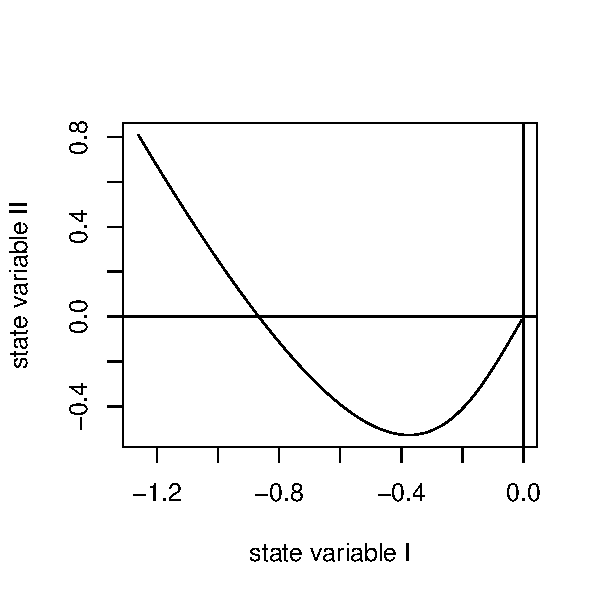
\includegraphics[width=\maxwidth]{figure/solveA} 

\end{knitrout}

\section{Vector field plots}

Another way to get more insight into the model that is not dependent
on specific initial conditions is to construct a vector field plot,
which represents the magnitude and direction of the time derivative at
various points in the state space.  To construct a vector field plot
we use the code{plotrix} package,
\begin{knitrout}
\definecolor{shadecolor}{rgb}{0.969, 0.969, 0.969}\color{fgcolor}\begin{kframe}
\begin{alltt}
\hlkwd{install.package}\hlstd{(}\hlstr{"plotrix"}\hlstd{)}
\hlkwd{library}\hlstd{(plotrix)}
\end{alltt}
\end{kframe}
\end{knitrout}
\begin{knitrout}
\definecolor{shadecolor}{rgb}{0.969, 0.969, 0.969}\color{fgcolor}\begin{kframe}
\begin{alltt}
\hlkwd{library}\hlstd{(plotrix)}
\hlstd{xx} \hlkwb{<-} \hlkwd{seq}\hlstd{(}\hlopt{-}\hlnum{2}\hlstd{,} \hlnum{2}\hlstd{,} \hlkwc{length} \hlstd{=} \hlnum{10}\hlstd{)}
\hlstd{X} \hlkwb{<-} \hlkwd{as.matrix}\hlstd{(}\hlkwd{expand.grid}\hlstd{(xx, xx))}
\hlstd{Ax} \hlkwb{<-} \hlstd{X} \hlopt \hlkwd{t}\hlstd{(A)}
\hlkwd{par}\hlstd{(}\hlkwc{mar} \hlstd{=} \hlkwd{c}\hlstd{(}\hlnum{3}\hlstd{,} \hlnum{3}\hlstd{,} \hlnum{1}\hlstd{,} \hlnum{1}\hlstd{))}
\hlkwd{plot}\hlstd{(}\hlkwd{c}\hlstd{(}\hlopt{-}\hlnum{2}\hlstd{,} \hlnum{2}\hlstd{),} \hlkwd{c}\hlstd{(}\hlopt{-}\hlnum{2}\hlstd{,} \hlnum{2}\hlstd{),} \hlkwc{type} \hlstd{=} \hlstr{"n"}\hlstd{,}
     \hlkwc{las} \hlstd{=} \hlnum{1}\hlstd{)}
\hlkwd{abline}\hlstd{(}\hlkwc{h} \hlstd{=} \hlnum{0}\hlstd{,} \hlkwc{v} \hlstd{=} \hlnum{0}\hlstd{,} \hlkwc{lwd} \hlstd{=} \hlnum{0.5}\hlstd{)}
\hlkwd{vectorField}\hlstd{(Ax[,}\hlnum{1}\hlstd{], Ax[,}\hlnum{2}\hlstd{],}
            \hlstd{X[,}\hlnum{1}\hlstd{], X[,}\hlnum{2}\hlstd{])}
\hlstd{eigA} \hlkwb{<-} \hlkwd{eigen}\hlstd{(A)}
\hlstd{eVec} \hlkwb{<-} \hlstd{eigA}\hlopt{$}\hlstd{vectors}
\hlstd{eVecInv} \hlkwb{<-} \hlkwd{solve}\hlstd{(eVec)}
\hlstd{eVal} \hlkwb{<-} \hlstd{eigA}\hlopt{$}\hlstd{values}
\hlstd{eigSlopes} \hlkwb{<-} \hlstd{eVec[}\hlnum{2}\hlstd{,]}\hlopt{/}\hlstd{eVec[}\hlnum{1}\hlstd{,]}
\hlkwd{abline}\hlstd{(}\hlkwc{a} \hlstd{=} \hlnum{0}\hlstd{,}
       \hlkwc{b} \hlstd{= eigSlopes[}\hlnum{1}\hlstd{],}
       \hlkwc{col} \hlstd{=} \hlstr{"red"}\hlstd{)}
\hlkwd{abline}\hlstd{(}\hlkwc{a} \hlstd{=} \hlnum{0}\hlstd{,}
       \hlkwc{b} \hlstd{= eigSlopes[}\hlnum{2}\hlstd{],}
       \hlkwc{col} \hlstd{=} \hlstr{"blue"}\hlstd{)}
\hlkwd{lines}\hlstd{(x,} \hlkwc{col} \hlstd{=} \hlstr{"green"}\hlstd{,} \hlkwc{lwd} \hlstd{=} \hlnum{3}\hlstd{)}
\end{alltt}
\end{kframe}
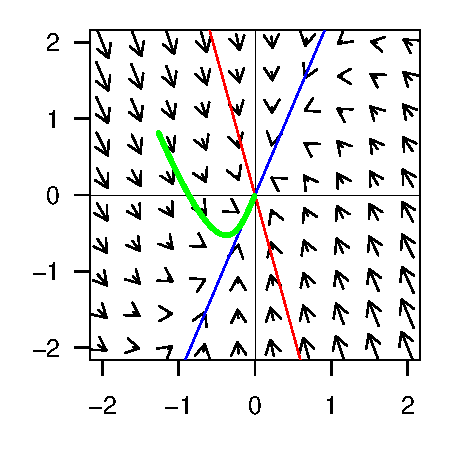
\includegraphics[width=\maxwidth]{figure/vectorField} 

\end{knitrout}
\noindent We have also plotted the two eigenvectors (in red and blue)
and the trajectory (in green).  Note that the vectors along the
eigenvectors point to the fixed point, indicating stability.

\textbf{Exercise\exnumber}: Choose different values for \code{A} and
explore the range of behaviour that is possible with bivariate linear
models.  Choose values untill you have found (1) models with cycles,
(2) models with only one linearly independent eigenvector, and (3)
models with one positive and one negative eigenvalue.

\section{Numerical solutions to differential equations}

\R\ can also be used to solve differential equations.  You are
required to be able to use \R\ for this purpose, but not until we
cover them in lectures.  We will be using the \code{deSolve} add-on
package for \R, which can be obtained by,
\begin{knitrout}
\definecolor{shadecolor}{rgb}{0.969, 0.969, 0.969}\color{fgcolor}\begin{kframe}
\begin{alltt}
\hlkwd{install.package}\hlstd{(}\hlstr{"deSolve"}\hlstd{)}
\hlkwd{library}\hlstd{(deSolve)}
\end{alltt}
\end{kframe}
\end{knitrout}


To illustrate \code{deSolve} we will use the logistic model,
\begin{equation}
  \label{eq:1}
  \frac{dN}{dt} = rN\left(1-\frac{N}{K}\right)
\end{equation}
The first task is to construct a function that computes the gradient
(i.e. the time-derivative of the state variable),
\begin{knitrout}
\definecolor{shadecolor}{rgb}{0.969, 0.969, 0.969}\color{fgcolor}\begin{kframe}
\begin{alltt}
\hlstd{gradfun} \hlkwb{<-} \hlkwa{function}\hlstd{(}\hlkwc{t}\hlstd{,} \hlkwc{N}\hlstd{,} \hlkwc{params}\hlstd{) \{}
    \hlkwd{with}\hlstd{(}\hlkwd{c}\hlstd{(}\hlkwd{as.list}\hlstd{(N),} \hlkwd{as.list}\hlstd{(params)),}
         \hlkwd{list}\hlstd{(}\hlkwc{N} \hlstd{= r} \hlopt{*} \hlstd{N} \hlopt{*} \hlstd{(}\hlnum{1} \hlopt{-} \hlstd{N}\hlopt{/}\hlstd{K)))}
\hlstd{\}}
\end{alltt}
\end{kframe}
\end{knitrout}
\noindent This function takes three arguments, \code{t}, which accepts
a time point at which to evaluate the differential equation, \code{N},
which accepts the state variable (e.g. $N$), and \code{params}, which
accepts the model parameters (e.g. $r$ and $K$).  The arguments must
be in this order, but the names do not matter.  Note also that we have
used the \code{with} function, which at this point might seem a bit
magical, but allows us to refer to the state variables and parameters
by name.  The output of this function is an \R\ list with the gradient
as the first argument.  The \code{NULL} element must be present as a
placeholder.

To solve this function, we use the \code{lsoda} function,
\begin{knitrout}
\definecolor{shadecolor}{rgb}{0.969, 0.969, 0.969}\color{fgcolor}\begin{kframe}
\begin{alltt}
\hlstd{desol} \hlkwb{<-} \hlkwd{lsoda}\hlstd{(}\hlkwc{y} \hlstd{=} \hlkwd{c}\hlstd{(}\hlkwc{N} \hlstd{=} \hlnum{0.1}\hlstd{),}
               \hlkwc{times} \hlstd{=} \hlkwd{seq}\hlstd{(}\hlnum{0}\hlstd{,} \hlnum{10}\hlstd{,} \hlkwc{by} \hlstd{=} \hlnum{0.1}\hlstd{),}
               \hlkwc{func} \hlstd{= gradfun,}
               \hlkwc{parms} \hlstd{=} \hlkwd{c}\hlstd{(}\hlkwc{r} \hlstd{=} \hlnum{1}\hlstd{,} \hlkwc{K} \hlstd{=} \hlnum{5}\hlstd{))}
\end{alltt}
\end{kframe}
\end{knitrout}
which takes the initial values, \code{y}, the times at which to
evaluate, \code{times}, the gradient function, \code{func}, and
numerical values for the parameters, \code{parms}.  Let's look at the
solutions for the first few time points,
\begin{knitrout}
\definecolor{shadecolor}{rgb}{0.969, 0.969, 0.969}\color{fgcolor}\begin{kframe}
\begin{alltt}
\hlstd{desol} \hlkwb{<-} \hlkwd{as.data.frame}\hlstd{(desol)}
\hlkwd{head}\hlstd{(desol)}
\end{alltt}
\begin{verbatim}
##   time      N
## 1  0.0 0.1000
## 2  0.1 0.1103
## 3  0.2 0.1216
## 4  0.3 0.1340
## 5  0.4 0.1477
## 6  0.5 0.1628
\end{verbatim}
\end{kframe}
\end{knitrout}
We may plot the results using \code{with} as well,
\begin{knitrout}
\definecolor{shadecolor}{rgb}{0.969, 0.969, 0.969}\color{fgcolor}\begin{kframe}
\begin{alltt}
\hlkwd{par}\hlstd{(}\hlkwc{mar} \hlstd{=} \hlkwd{c}\hlstd{(}\hlnum{4}\hlstd{,} \hlnum{4}\hlstd{,} \hlnum{1}\hlstd{,} \hlnum{1}\hlstd{))}
\hlkwd{with}\hlstd{(desol,} \hlkwd{plot}\hlstd{(time, N,}
                 \hlkwc{las} \hlstd{=} \hlnum{1}\hlstd{,}
                 \hlkwc{type} \hlstd{=} \hlstr{"l"}\hlstd{))}
\end{alltt}
\end{kframe}
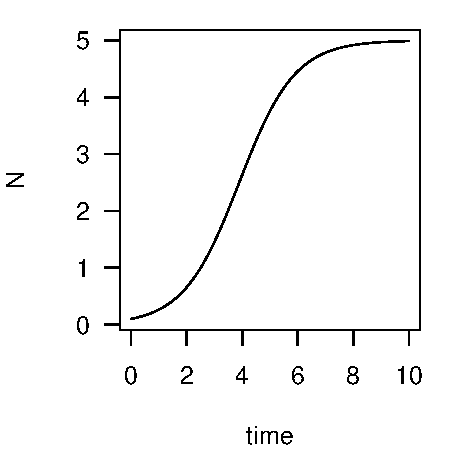
\includegraphics[width=\maxwidth]{figure/unnamed-chunk-7} 

\end{knitrout}

The \code{deSolve} package may also be used to solve multivariate
differential equations.  Please consult the \code{?lsoda} help file
for examples.

\textbf{Exercise\exnumber *}: Use the techniques you have learnt to
complete Project 5.9 on pp.320-1 in MS.  For part b, contruct a vector
field plot instead of a phase plane analysis.

\bibliography{lab1.bib}
\bibliographystyle{plain}

\end{document}
